\documentclass[ignorenonframetext,]{beamer}
\usepackage{amssymb,amsmath}
\usepackage{ifxetex,ifluatex}
\usepackage{fixltx2e} % provides \textsubscript
\usepackage{lmodern}
\ifxetex
  \usepackage{fontspec,xltxtra,xunicode}
  \defaultfontfeatures{Mapping=tex-text,Scale=MatchLowercase}
  \newcommand{\euro}{€}
\else
  \ifluatex
    \usepackage{fontspec}
    \defaultfontfeatures{Mapping=tex-text,Scale=MatchLowercase}
    \newcommand{\euro}{€}
  \else
    \usepackage[T1]{fontenc}
    \usepackage[utf8]{inputenc}
      \fi
\fi
\IfFileExists{upquote.sty}{\usepackage{upquote}}{}
% use microtype if available
\IfFileExists{microtype.sty}{\usepackage{microtype}}{}
\usepackage{color}
\usepackage{fancyvrb}
\newcommand{\VerbBar}{|}
\newcommand{\VERB}{\Verb[commandchars=\\\{\}]}
\DefineVerbatimEnvironment{Highlighting}{Verbatim}{commandchars=\\\{\}}
% Add ',fontsize=\small' for more characters per line
\usepackage{framed}
\definecolor{shadecolor}{RGB}{248,248,248}
\newenvironment{Shaded}{\begin{snugshade}}{\end{snugshade}}
\newcommand{\KeywordTok}[1]{\textcolor[rgb]{0.13,0.29,0.53}{\textbf{{#1}}}}
\newcommand{\DataTypeTok}[1]{\textcolor[rgb]{0.13,0.29,0.53}{{#1}}}
\newcommand{\DecValTok}[1]{\textcolor[rgb]{0.00,0.00,0.81}{{#1}}}
\newcommand{\BaseNTok}[1]{\textcolor[rgb]{0.00,0.00,0.81}{{#1}}}
\newcommand{\FloatTok}[1]{\textcolor[rgb]{0.00,0.00,0.81}{{#1}}}
\newcommand{\CharTok}[1]{\textcolor[rgb]{0.31,0.60,0.02}{{#1}}}
\newcommand{\StringTok}[1]{\textcolor[rgb]{0.31,0.60,0.02}{{#1}}}
\newcommand{\CommentTok}[1]{\textcolor[rgb]{0.56,0.35,0.01}{\textit{{#1}}}}
\newcommand{\OtherTok}[1]{\textcolor[rgb]{0.56,0.35,0.01}{{#1}}}
\newcommand{\AlertTok}[1]{\textcolor[rgb]{0.94,0.16,0.16}{{#1}}}
\newcommand{\FunctionTok}[1]{\textcolor[rgb]{0.00,0.00,0.00}{{#1}}}
\newcommand{\RegionMarkerTok}[1]{{#1}}
\newcommand{\ErrorTok}[1]{\textbf{{#1}}}
\newcommand{\NormalTok}[1]{{#1}}
\usepackage{url}
\usepackage{letltxmacro}
\makeatletter
\def\maxwidth{\ifdim\Gin@nat@width>\linewidth\linewidth\else\Gin@nat@width\fi}
\def\maxheight{\ifdim\Gin@nat@height>\textheight0.8\textheight\else\Gin@nat@height\fi}
\makeatother
\AtBeginDocument{
  \LetLtxMacro\Oldincludegraphics\includegraphics
  \renewcommand{\includegraphics}[2][]{%
    \Oldincludegraphics[#1,width=\maxwidth,height=\maxheight,keepaspectratio]{#2}}
}

% Comment these out if you don't want a slide with just the
% part/section/subsection/subsubsection title:
\AtBeginPart{
  \let\insertpartnumber\relax
  \let\partname\relax
  \frame{\partpage}
}
\AtBeginSection{
  \let\insertsectionnumber\relax
  \let\sectionname\relax
  \frame{\sectionpage}
}
\AtBeginSubsection{
  \let\insertsubsectionnumber\relax
  \let\subsectionname\relax
  \frame{\subsectionpage}
}

\setlength{\parindent}{0pt}
\setlength{\parskip}{6pt plus 2pt minus 1pt}
\setlength{\emergencystretch}{3em}  % prevent overfull lines
\setcounter{secnumdepth}{0}

\title{Intro to Grammar of Graphics (ggplot2)}
\author{Jason Bryer}
\date{September 9, 2014}

\begin{document}
\frame{\titlepage}

\begin{frame}{ggplot2}

\texttt{ggplot2} (Wickham, 2009) is an R package that implements the
\emph{Graammar of Graphics} introduced by Wilkinson (2005).

(Journal of Statistical Software
paper){[}\url{http://www.jstatsoft.org/v17/b03/paper}{]}

\end{frame}

\begin{frame}[fragile]{The Lego Package}

\begin{Shaded}
\begin{Highlighting}[]
\CommentTok{# https://github.com/seankross/lego}
\NormalTok{devtools::}\KeywordTok{install_github}\NormalTok{(}\StringTok{"seankross/lego"}\NormalTok{)}
\end{Highlighting}
\end{Shaded}

\begin{Shaded}
\begin{Highlighting}[]
\KeywordTok{library}\NormalTok{(lego)}
\KeywordTok{library}\NormalTok{(psych)}
\end{Highlighting}
\end{Shaded}

\end{frame}

\begin{frame}[fragile]{The Lego Package}

\begin{Shaded}
\begin{Highlighting}[]
\KeywordTok{data}\NormalTok{(legosets)}
\KeywordTok{head}\NormalTok{(legosets, }\DataTypeTok{n=}\DecValTok{3}\NormalTok{)}
\end{Highlighting}
\end{Shaded}

\begin{verbatim}
##   Item_Number                 Name Year           Theme
## 1       10241 Maersk Line Triple-E 2014 Advanced Models
## 2       10242   Mini Cooper MK VII 2014 Advanced Models
## 3       10243  Parisian Restaurant 2014 Advanced Models
##            Subtheme Pieces Minifigures
## 1            Maersk   1518          NA
## 2          Vehicles   1077          NA
## 3 Modular Buildings   2469           5
##                                               Image_URL GBP_MSRP
## 1 http://www.1000steine.com/brickset/images/10241-1.jpg   109.99
## 2 http://www.1000steine.com/brickset/images/10242-1.jpg    74.99
## 3 http://www.1000steine.com/brickset/images/10243-1.jpg   132.99
##   USD_MSRP CAD_MSRP EUR_MSRP Packaging   Availability
## 1   149.99      180   129.99       Box LEGO exclusive
## 2    99.99      120    89.99       Box LEGO exclusive
## 3   159.99      190   149.99       Box LEGO exclusive
\end{verbatim}

\end{frame}

\begin{frame}{Parts of a ggplot2 statement}

\begin{itemize}[<+->]
\itemsep1pt\parskip0pt\parsep0pt
\item
  Data\\ ggplot(myDataFrame, aes(x=x, y=y)
\item
  Layers\\ geom\_point(), geom\_histogram()
\item
  Facets\\ facet\_wrap(\textasciitilde{} cut),
  facet\_grid(\textasciitilde{} cut)
\item
  Scales\\ scale\_y\_log10()
\item
  Other options\\ ggtitle(`my title'), ylim(c(0, 10000)), xlab(`x-axis
  label')
\end{itemize}

\end{frame}

\begin{frame}[fragile]{There are Lots of Geoms}

\begin{Shaded}
\begin{Highlighting}[]
\KeywordTok{ls}\NormalTok{(}\StringTok{"package:ggplot2"}\NormalTok{)[}\KeywordTok{substr}\NormalTok{(}\KeywordTok{ls}\NormalTok{(}\StringTok{"package:ggplot2"}\NormalTok{), }
                             \DecValTok{1}\NormalTok{, }\DecValTok{5}\NormalTok{) ==}\StringTok{ 'geom_'}\NormalTok{]}
\end{Highlighting}
\end{Shaded}

\begin{verbatim}
##  [1] "geom_abline"     "geom_area"       "geom_bar"       
##  [4] "geom_bin2d"      "geom_blank"      "geom_boxplot"   
##  [7] "geom_contour"    "geom_crossbar"   "geom_density"   
## [10] "geom_density2d"  "geom_dotplot"    "geom_errorbar"  
## [13] "geom_errorbarh"  "geom_freqpoly"   "geom_hex"       
## [16] "geom_histogram"  "geom_hline"      "geom_jitter"    
## [19] "geom_line"       "geom_linerange"  "geom_map"       
## [22] "geom_path"       "geom_point"      "geom_pointrange"
## [25] "geom_polygon"    "geom_quantile"   "geom_raster"    
## [28] "geom_rect"       "geom_ribbon"     "geom_rug"       
## [31] "geom_segment"    "geom_smooth"     "geom_step"      
## [34] "geom_text"       "geom_tile"       "geom_violin"    
## [37] "geom_vline"
\end{verbatim}

\end{frame}

\begin{frame}[fragile]{Histograms}

\begin{Shaded}
\begin{Highlighting}[]
\KeywordTok{ggplot}\NormalTok{(legosets, }\KeywordTok{aes}\NormalTok{(}\DataTypeTok{x=}\NormalTok{Pieces)) +}\StringTok{ }
\StringTok{    }\KeywordTok{geom_histogram}\NormalTok{()}
\end{Highlighting}
\end{Shaded}

\begin{verbatim}
## stat_bin: binwidth defaulted to range/30. Use 'binwidth = x' to adjust this.
\end{verbatim}

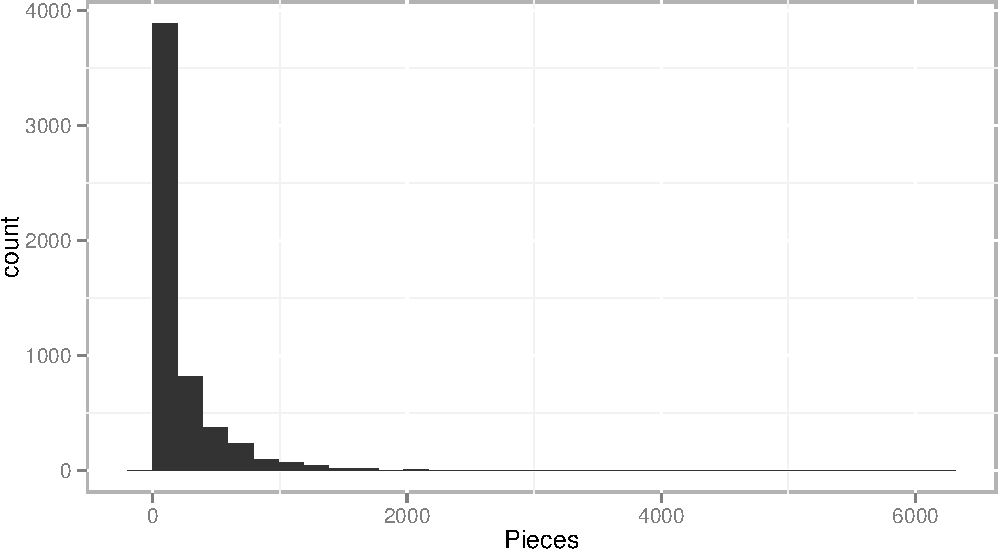
\includegraphics{./ggplot2_files/figure-beamer/unnamed-chunk-2.pdf}

\end{frame}

\begin{frame}[fragile]{Log Transformations}

\begin{Shaded}
\begin{Highlighting}[]
\KeywordTok{ggplot}\NormalTok{(legosets, }\KeywordTok{aes}\NormalTok{(}\DataTypeTok{x=}\NormalTok{Pieces)) +}\StringTok{ }
\StringTok{    }\KeywordTok{geom_histogram}\NormalTok{() +}\StringTok{ }\KeywordTok{scale_x_log10}\NormalTok{()}
\end{Highlighting}
\end{Shaded}

\begin{verbatim}
## stat_bin: binwidth defaulted to range/30. Use 'binwidth = x' to adjust this.
\end{verbatim}

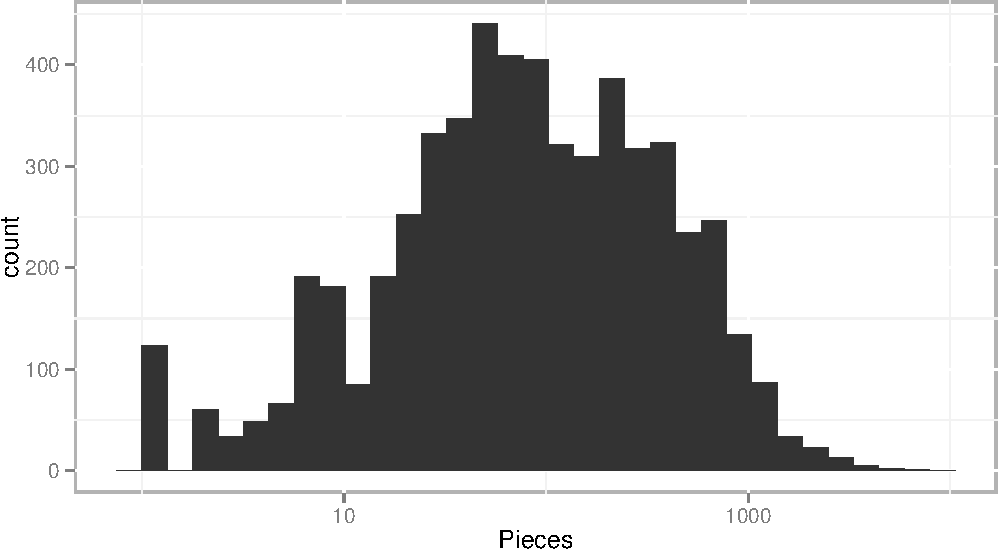
\includegraphics{./ggplot2_files/figure-beamer/unnamed-chunk-3.pdf}

\end{frame}

\begin{frame}[fragile]{Barplots}

\begin{Shaded}
\begin{Highlighting}[]
\KeywordTok{ggplot}\NormalTok{(legosets, }\KeywordTok{aes}\NormalTok{(}\DataTypeTok{x=}\NormalTok{Theme)) +}\StringTok{ }\KeywordTok{geom_bar}\NormalTok{() +}\StringTok{ }
\StringTok{    }\KeywordTok{theme}\NormalTok{(}\DataTypeTok{axis.text.x=}\KeywordTok{element_text}\NormalTok{(}\DataTypeTok{angle=}\DecValTok{90}\NormalTok{))}
\end{Highlighting}
\end{Shaded}

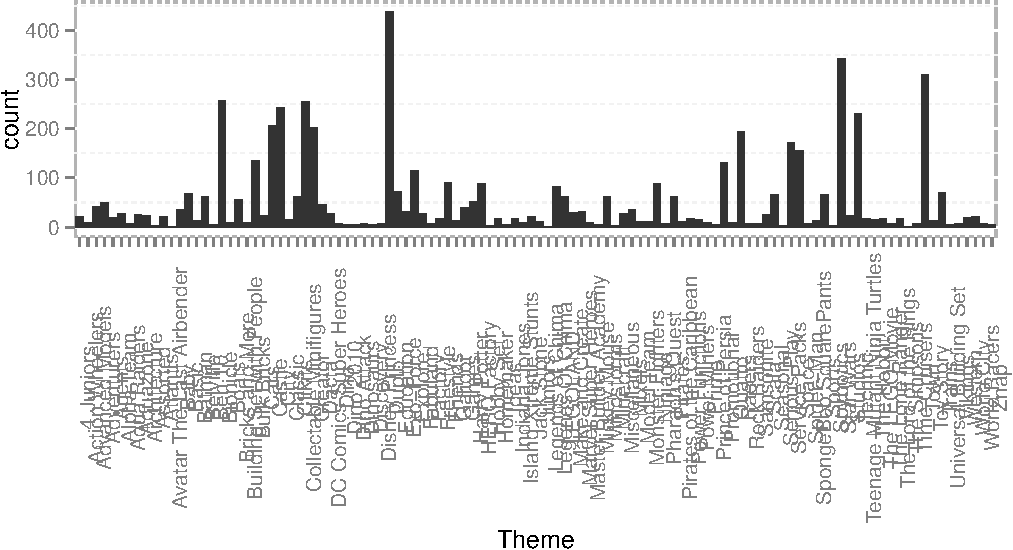
\includegraphics{./ggplot2_files/figure-beamer/unnamed-chunk-4.pdf}

\end{frame}

\begin{frame}[fragile]{Barplots Flipping Coordinates}

\begin{Shaded}
\begin{Highlighting}[]
\KeywordTok{ggplot}\NormalTok{(legosets, }\KeywordTok{aes}\NormalTok{(}\DataTypeTok{x=}\NormalTok{Theme)) +}\StringTok{ }\KeywordTok{geom_bar}\NormalTok{() +}\StringTok{ }
\StringTok{    }\KeywordTok{coord_flip}\NormalTok{()}
\end{Highlighting}
\end{Shaded}

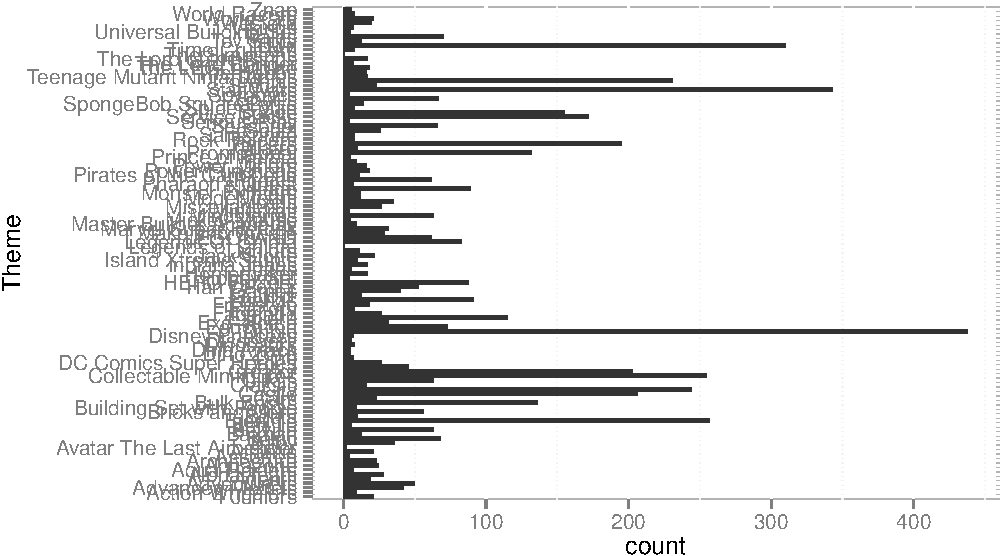
\includegraphics{./ggplot2_files/figure-beamer/unnamed-chunk-5.pdf}

\end{frame}

\begin{frame}[fragile]{Labeling Barplots}

\begin{Shaded}
\begin{Highlighting}[]
\NormalTok{df <-}\StringTok{ }\KeywordTok{as.data.frame}\NormalTok{(}\KeywordTok{table}\NormalTok{(legosets$Theme))}
\NormalTok{df <-}\StringTok{ }\NormalTok{df[df$Freq >}\StringTok{ }\DecValTok{20}\NormalTok{,]}
\KeywordTok{ggplot}\NormalTok{(df, }\KeywordTok{aes}\NormalTok{(}\DataTypeTok{x=}\NormalTok{Var1, }\DataTypeTok{y=}\NormalTok{Freq, }\DataTypeTok{label=}\NormalTok{Freq)) +}\StringTok{ }
\StringTok{    }\KeywordTok{geom_bar}\NormalTok{(}\DataTypeTok{stat=}\StringTok{'identity'}\NormalTok{, }\DataTypeTok{alpha=}\NormalTok{.}\DecValTok{5}\NormalTok{) +}\StringTok{ }
\StringTok{    }\KeywordTok{coord_flip}\NormalTok{() +}\StringTok{ }\KeywordTok{geom_text}\NormalTok{(}\DataTypeTok{hjust=}\DecValTok{0}\NormalTok{)}
\end{Highlighting}
\end{Shaded}

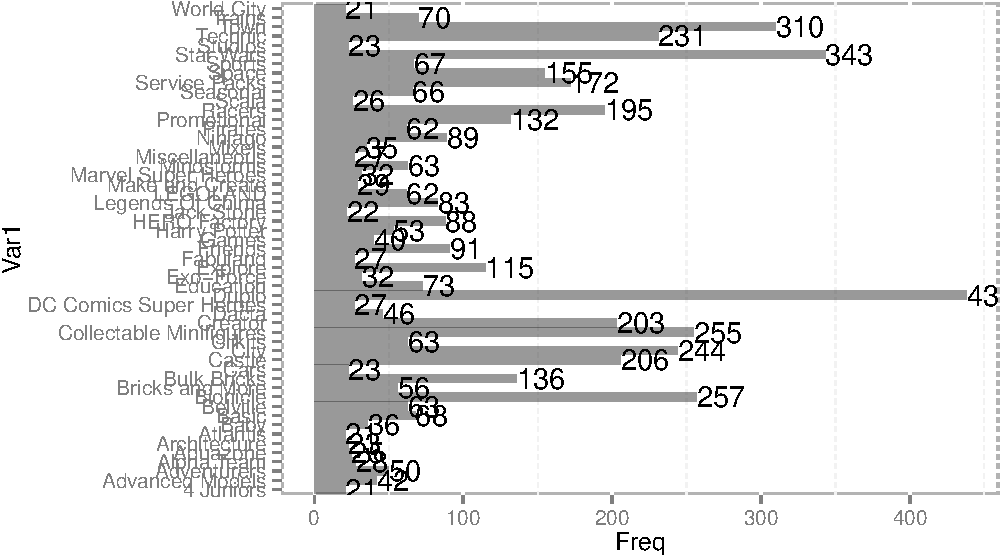
\includegraphics{./ggplot2_files/figure-beamer/unnamed-chunk-6.pdf}

\end{frame}

\begin{frame}[fragile]{Boxplots}

\begin{Shaded}
\begin{Highlighting}[]
\KeywordTok{ggplot}\NormalTok{(legosets, }\KeywordTok{aes}\NormalTok{(}\DataTypeTok{x=}\NormalTok{Availability, Pieces)) +}\StringTok{ }
\StringTok{    }\KeywordTok{geom_boxplot}\NormalTok{()}
\end{Highlighting}
\end{Shaded}

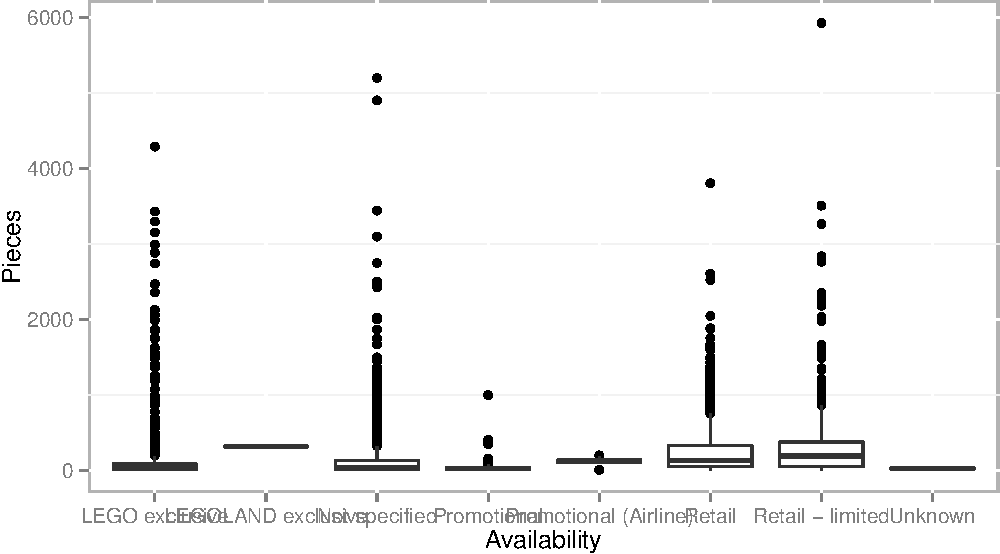
\includegraphics{./ggplot2_files/figure-beamer/unnamed-chunk-7.pdf}

\end{frame}

\begin{frame}[fragile]{Boxplots Flipping Coordinates}

\begin{Shaded}
\begin{Highlighting}[]
\KeywordTok{ggplot}\NormalTok{(legosets, }\KeywordTok{aes}\NormalTok{(}\DataTypeTok{x=}\NormalTok{Availability, Pieces)) +}\StringTok{ }
\StringTok{    }\KeywordTok{geom_boxplot}\NormalTok{() +}\StringTok{ }\KeywordTok{coord_flip}\NormalTok{()}
\end{Highlighting}
\end{Shaded}

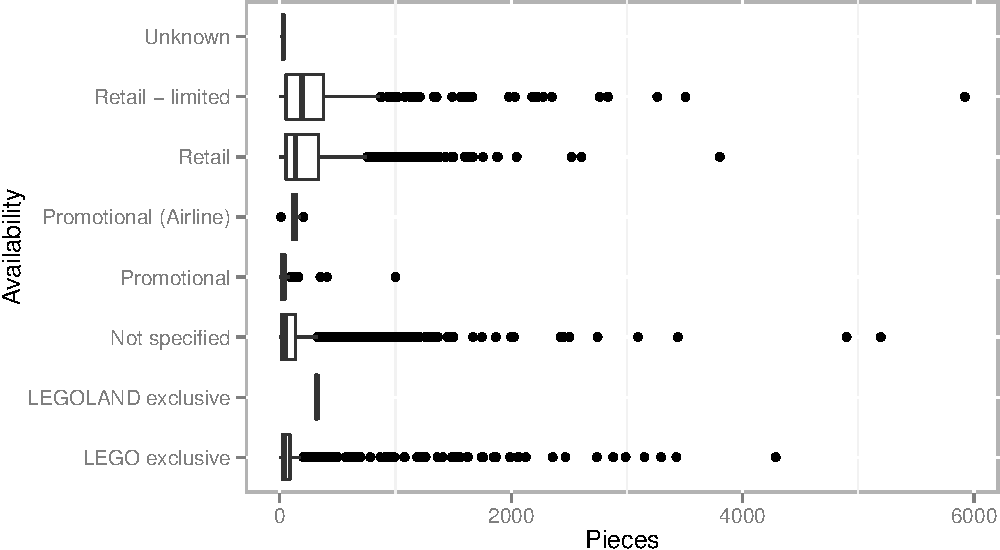
\includegraphics{./ggplot2_files/figure-beamer/unnamed-chunk-8.pdf}

\end{frame}

\begin{frame}[fragile]{Boxplots for Longitudinal Data}

\begin{Shaded}
\begin{Highlighting}[]
\KeywordTok{ggplot}\NormalTok{(legosets, }\KeywordTok{aes}\NormalTok{(}\DataTypeTok{x=}\KeywordTok{factor}\NormalTok{(Year), }\DataTypeTok{y=}\NormalTok{USD_MSRP)) +}\StringTok{ }
\StringTok{    }\KeywordTok{geom_boxplot}\NormalTok{() +}\StringTok{ }\KeywordTok{theme}\NormalTok{(}\DataTypeTok{axis.text.x=}\KeywordTok{element_text}\NormalTok{(}\DataTypeTok{angle=}\DecValTok{90}\NormalTok{)) +}\StringTok{ }
\StringTok{    }\KeywordTok{xlab}\NormalTok{(}\StringTok{'Year'}\NormalTok{) +}\StringTok{ }\KeywordTok{ylab}\NormalTok{(}\StringTok{'Price'}\NormalTok{)}
\end{Highlighting}
\end{Shaded}

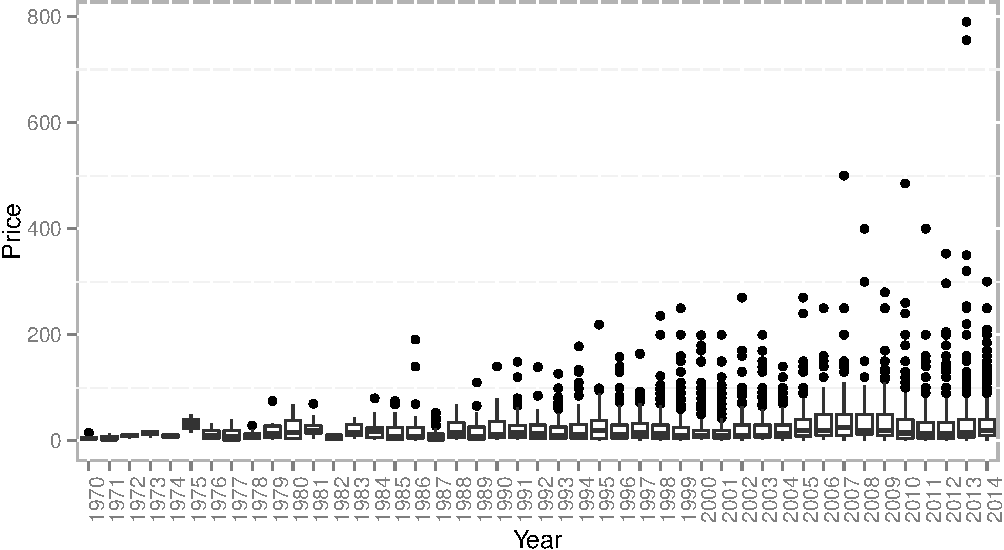
\includegraphics{./ggplot2_files/figure-beamer/unnamed-chunk-9.pdf}

\end{frame}

\begin{frame}[fragile]{Scatterplots}

\begin{Shaded}
\begin{Highlighting}[]
\KeywordTok{ggplot}\NormalTok{(legosets, }\KeywordTok{aes}\NormalTok{(}\DataTypeTok{x=}\NormalTok{Pieces, }\DataTypeTok{y=}\NormalTok{USD_MSRP)) +}\StringTok{ }
\StringTok{    }\KeywordTok{geom_point}\NormalTok{(}\DataTypeTok{alhpa=}\NormalTok{.}\DecValTok{5}\NormalTok{)}
\end{Highlighting}
\end{Shaded}

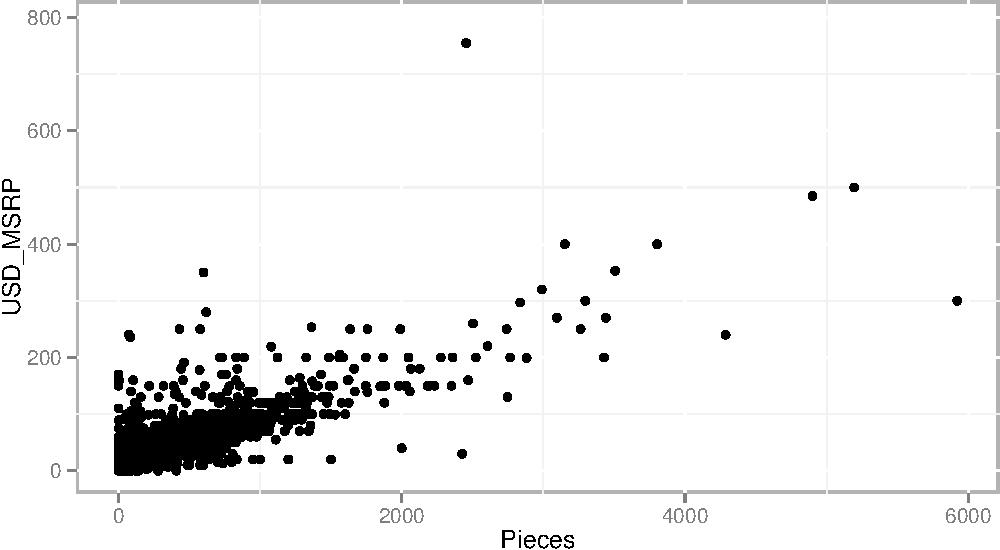
\includegraphics{./ggplot2_files/figure-beamer/unnamed-chunk-10.pdf}

\end{frame}

\begin{frame}[fragile]{Scatterplots with Loess Plots}

\begin{Shaded}
\begin{Highlighting}[]
\KeywordTok{ggplot}\NormalTok{(legosets, }\KeywordTok{aes}\NormalTok{(}\DataTypeTok{x=}\NormalTok{Pieces, }\DataTypeTok{y=}\NormalTok{USD_MSRP)) +}\StringTok{ }
\StringTok{    }\KeywordTok{geom_point}\NormalTok{(}\DataTypeTok{alhpa=}\NormalTok{.}\DecValTok{5}\NormalTok{) +}\StringTok{ }\KeywordTok{geom_smooth}\NormalTok{()}
\end{Highlighting}
\end{Shaded}

\begin{verbatim}
## geom_smooth: method="auto" and size of largest group is >=1000, so using gam with formula: y ~ s(x, bs = "cs"). Use 'method = x' to change the smoothing method.
\end{verbatim}

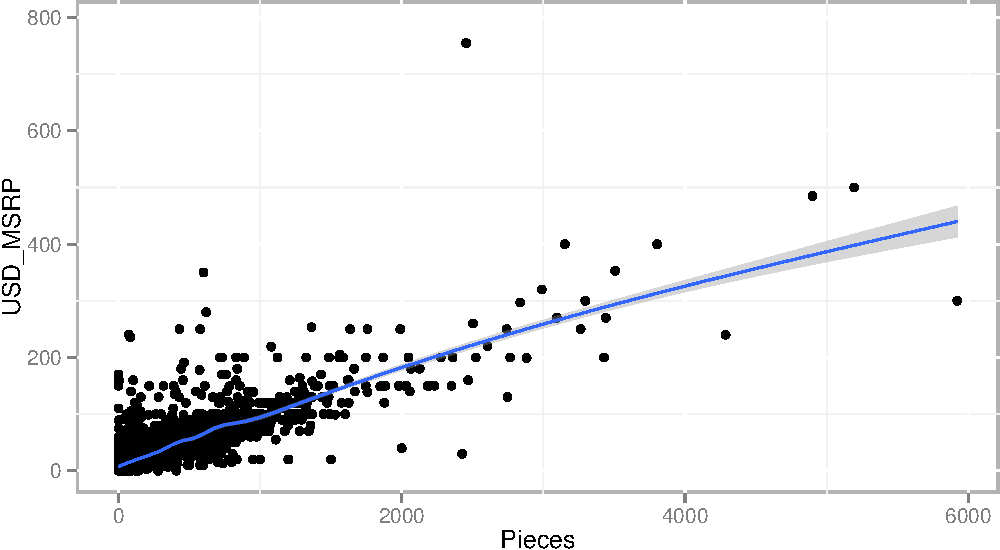
\includegraphics{./ggplot2_files/figure-beamer/unnamed-chunk-11.pdf}

\end{frame}

\end{document}
